\documentclass[tikz,border=4pt]{standalone}
\usepackage{fontspec}
\setmainfont{Times New Roman}
\usepackage{amsmath,amssymb}
\usepackage{xcolor}
\usetikzlibrary{arrows.meta,positioning,shapes.geometric,fit,backgrounds,calc}

\begin{document}
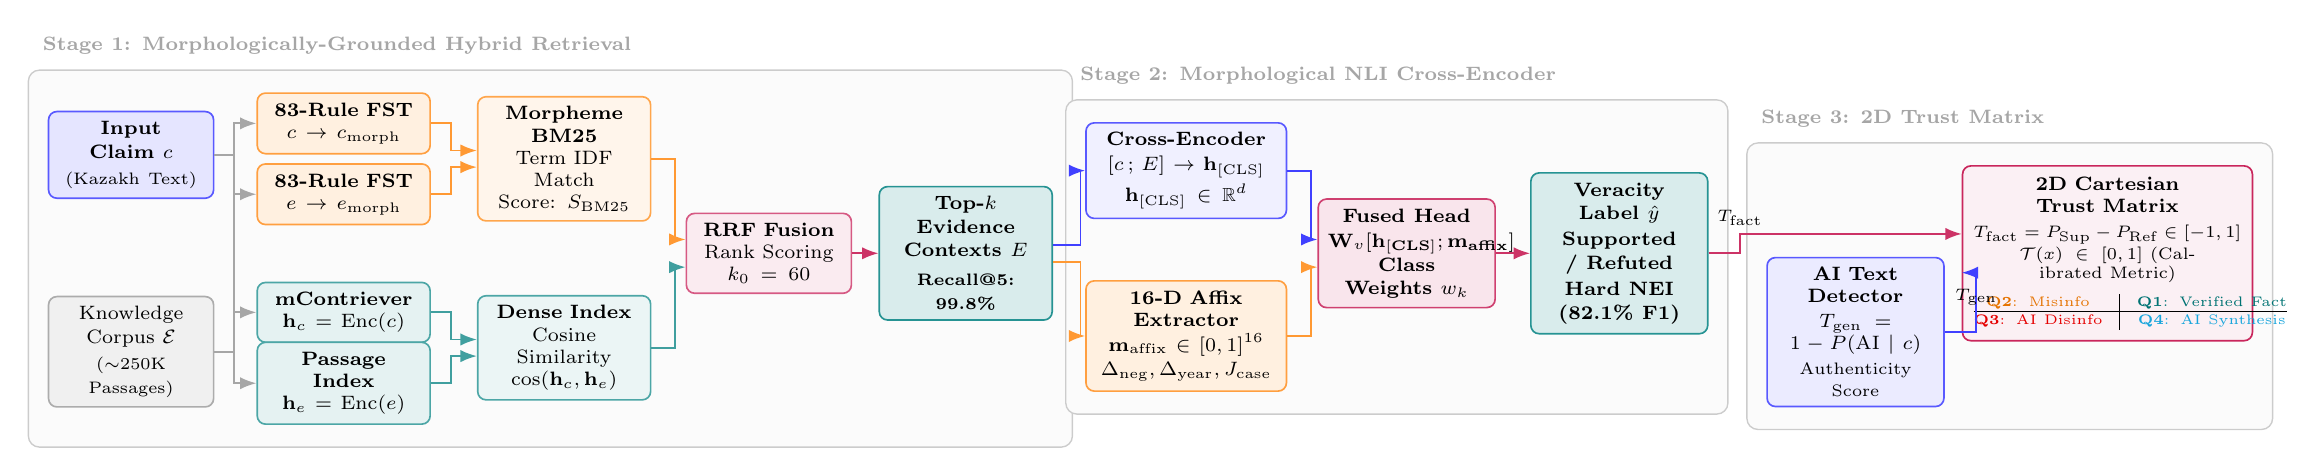
\begin{tikzpicture}[
    >=Latex,
    line width=0.6pt,
    % Node styles with explicit text width and padding
    box/.style={
        rectangle, 
        draw=gray!70, 
        fill=white, 
        rounded corners=3pt, 
        align=center, 
        line width=0.6pt, 
        inner sep=3.5pt
    },
    inbox/.style={
        box, 
        fill=blue!10, 
        draw=blue!65, 
        text width=1.85cm, 
        font=\fontsize{7pt}{8.5pt}\selectfont\bfseries
    },
    corpusbox/.style={
        box, 
        fill=gray!12, 
        draw=gray!65, 
        text width=1.85cm, 
        font=\fontsize{7pt}{8.5pt}\selectfont
    },
    fststyle/.style={
        box, 
        fill=orange!12, 
        draw=orange!75, 
        text width=1.95cm, 
        font=\fontsize{6.8pt}{8pt}\selectfont
    },
    densestyle/.style={
        box, 
        fill=teal!10, 
        draw=teal!70, 
        text width=1.95cm, 
        font=\fontsize{6.8pt}{8pt}\selectfont
    },
    bm25style/.style={
        box, 
        fill=orange!8, 
        draw=orange!70, 
        text width=1.95cm, 
        font=\fontsize{6.8pt}{8pt}\selectfont
    },
    simstyle/.style={
        box, 
        fill=teal!8, 
        draw=teal!70, 
        text width=1.95cm, 
        font=\fontsize{6.8pt}{8pt}\selectfont
    },
    rrfstyle/.style={
        box, 
        fill=purple!8, 
        draw=purple!65, 
        text width=1.85cm, 
        font=\fontsize{6.8pt}{8pt}\selectfont
    },
    evidencestyle/.style={
        box, 
        fill=teal!15, 
        draw=teal!85, 
        text width=1.95cm, 
        font=\fontsize{7pt}{8.5pt}\selectfont\bfseries
    },
    encstyle/.style={
        box, 
        fill=blue!6, 
        draw=blue!65, 
        text width=2.3cm, 
        font=\fontsize{6.8pt}{8pt}\selectfont
    },
    affixstyle/.style={
        box, 
        fill=orange!12, 
        draw=orange!75, 
        text width=2.3cm, 
        font=\fontsize{6.8pt}{8pt}\selectfont
    },
    headstyle/.style={
        box, 
        fill=purple!10, 
        draw=purple!75, 
        text width=2.0cm, 
        font=\fontsize{6.8pt}{8pt}\selectfont\bfseries
    },
    veracitystyle/.style={
        box, 
        fill=teal!15, 
        draw=teal!85, 
        text width=2.0cm, 
        font=\fontsize{7pt}{8.5pt}\selectfont\bfseries
    },
    aidetstyle/.style={
        box, 
        fill=blue!8, 
        draw=blue!65, 
        text width=2.0cm, 
        font=\fontsize{6.8pt}{8pt}\selectfont
    },
    matrixstyle/.style={
        box, 
        fill=purple!6, 
        draw=purple!85, 
        text width=3.4cm, 
        font=\fontsize{6.8pt}{8pt}\selectfont,
        inner sep=4pt
    },
    stagepanel/.style={
        rectangle, 
        draw=gray!40, 
        fill=gray!3, 
        rounded corners=4pt, 
        line width=0.5pt, 
        inner xsep=7pt, 
        inner ysep=8pt
    },
    stagetitle/.style={
        font=\fontsize{7.5pt}{9pt}\selectfont\bfseries, 
        text=gray!70, 
        anchor=south west
    },
    % Arrow styles
    arr/.style={->, line width=0.65pt, draw=gray!70},
    oarr/.style={->, line width=0.65pt, draw=orange!80},
    tarr/.style={->, line width=0.65pt, draw=teal!75},
    barr/.style={->, line width=0.65pt, draw=blue!75},
    parr/.style={->, line width=0.65pt, draw=purple!80}
]

% ==========================================
% STAGE 1: HYBRID EVIDENCE RETRIEVAL
% ==========================================
% Column 0: Inputs (X = 0.0)
\node[inbox] (claim_in) at (0.0, 1.25) {Input Claim $c$\\[1pt]\fontsize{5.8pt}{6.8pt}\selectfont\textmd{(Kazakh Text)}};
\node[corpusbox] (corpus_in) at (0.0, -1.25) {Knowledge Corpus $\mathcal{E}$\\[1pt]\fontsize{5.8pt}{6.8pt}\selectfont\textmd{($\sim$250K Passages)}};

% Column 1: Feature Processing (X = 2.7)
\node[fststyle] (fst_stem_c) at (2.7, 1.65) {\textbf{83-Rule FST}\\$c \to c_{\text{morph}}$};
\node[fststyle] (fst_stem_e) at (2.7, 0.75) {\textbf{83-Rule FST}\\$e \to e_{\text{morph}}$};
\node[densestyle] (dense_enc_c) at (2.7, -0.75) {\textbf{mContriever}\\$\mathbf{h}_c = \text{Enc}(c)$};
\node[densestyle] (dense_enc_e) at (2.7, -1.65) {\textbf{Passage Index}\\$\mathbf{h}_e = \text{Enc}(e)$};

% Column 2: Intermediate Retrieval (X = 5.5)
\node[bm25style] (bm25_node) at (5.5, 1.2) {\textbf{Morpheme BM25}\\Term IDF Match\\Score: $S_{\text{BM25}}$};
\node[simstyle] (dense_sim) at (5.5, -1.2) {\textbf{Dense Index}\\Cosine Similarity\\$\cos(\mathbf{h}_c, \mathbf{h}_e)$};

% Column 3: Fusion (X = 8.1)
\node[rrfstyle] (rrf_node) at (8.1, 0.0) {\textbf{RRF Fusion}\\Rank Scoring\\$k_0 = 60$};

% Column 4: Retrieved Context (X = 10.6)
\node[evidencestyle] (evidence_out) at (10.6, 0.0) {Top-$k$ Evidence\\Contexts $E$\\[2pt]\fontsize{6pt}{7pt}\selectfont Recall@5: 99.8\%};

% Arrows for Stage 1
\draw[arr] (claim_in.east) -- ++(0.25, 0) |- (fst_stem_c.west);
\draw[arr] (claim_in.east) -- ++(0.25, 0) |- (dense_enc_c.west);
\draw[arr] (corpus_in.east) -- ++(0.25, 0) |- (fst_stem_e.west);
\draw[arr] (corpus_in.east) -- ++(0.25, 0) |- (dense_enc_e.west);

\draw[oarr] (fst_stem_c.east) -- ++(0.25, 0) |- ([yshift=3pt]bm25_node.west);
\draw[oarr] (fst_stem_e.east) -- ++(0.25, 0) |- ([yshift=-3pt]bm25_node.west);
\draw[tarr] (dense_enc_c.east) -- ++(0.25, 0) |- ([yshift=3pt]dense_sim.west);
\draw[tarr] (dense_enc_e.east) -- ++(0.25, 0) |- ([yshift=-3pt]dense_sim.west);

\draw[oarr] (bm25_node.east) -- ++(0.3, 0) |- ([yshift=5pt]rrf_node.west);
\draw[tarr] (dense_sim.east) -- ++(0.3, 0) |- ([yshift=-5pt]rrf_node.west);
\draw[parr] (rrf_node.east) -- (evidence_out.west);

% ==========================================
% STAGE 2: MORPHOLOGICAL NLI CROSS-ENCODER
% ==========================================
% Column 5: Verifier Inputs (X = 13.4)
\node[encstyle] (xenc_node) at (13.4, 1.05) {\textbf{Cross-Encoder}\\[1pt]$[c \,;\, E] \to \mathbf{h}_{[\text{CLS}]}$\\[1pt]$\mathbf{h}_{[\text{CLS}]} \in \mathbb{R}^d$};
\node[affixstyle] (affix_node) at (13.4, -1.05) {\textbf{16-D Affix Extractor}\\[1pt]$\mathbf{m}_{\text{affix}} \in [0, 1]^{16}$\\[1pt]$\Delta_{\text{neg}}, \Delta_{\text{year}}, J_{\text{case}}$};

% Column 6: Classification Head (X = 16.2)
\node[headstyle] (fuse_head) at (16.2, 0.0) {\textbf{Fused Head}\\[1pt]$\mathbf{W}_v [\mathbf{h}_{[\text{CLS}]}; \mathbf{m}_{\text{affix}}]$\\[1pt]Class Weights $w_k$};

% Column 7: Veracity Output (X = 18.9)
\node[veracitystyle] (veracity_out) at (18.9, 0.0) {Veracity Label $\hat{y}$\\[1pt]Supported / Refuted\\[1pt]\textbf{Hard NEI (82.1\% F1)}};

% Arrows for Stage 2
\draw[barr] ([yshift=3pt]evidence_out.east) -- ++(0.35, 0) |- (xenc_node.west);
\draw[oarr] ([yshift=-3pt]evidence_out.east) -- ++(0.35, 0) |- (affix_node.west);

\draw[barr] (xenc_node.east) -- ++(0.3, 0) |- ([yshift=5pt]fuse_head.west);
\draw[oarr] (affix_node.east) -- ++(0.3, 0) |- ([yshift=-5pt]fuse_head.west);
\draw[parr] (fuse_head.east) -- (veracity_out.west);

% ==========================================
% STAGE 3: 2D TRUST MATRIX CALIBRATION
% ==========================================
% Column 8: AI Detector (X = 21.9)
\node[aidetstyle] (ai_det) at (21.9, -1.0) {\textbf{AI Text Detector}\\[1pt]$T_{\text{gen}} = 1 - P(\text{AI} \mid c)$\\[1pt]\fontsize{5.8pt}{6.8pt}\selectfont\textmd{Authenticity Score}};

% Column 9: 2D Trust Matrix (X = 25.1)
\node[matrixstyle] (trust_matrix_node) at (25.1, 0.0) {
    \textbf{2D Cartesian Trust Matrix}\\[2pt]
    \fontsize{6pt}{7pt}\selectfont
    $T_{\text{fact}} = P_{\text{Sup}} - P_{\text{Ref}} \in [-1, 1]$\\[1pt]
    $\mathcal{T}(x) \in [0, 1]$ (Calibrated Metric)\\[3pt]
    \fontsize{5.2pt}{6.2pt}\selectfont
    \begin{tabular}{@{}c|c@{}}
    \color{orange!90!black}\textbf{Q2}: Misinfo & \color{teal!90!black}\textbf{Q1}: Verified Fact \\ \hline
    \color{red!90!black}\textbf{Q3}: AI Disinfo & \color{cyan!90!black}\textbf{Q4}: AI Synthesis
    \end{tabular}
};

% Arrows for Stage 3
\draw[parr] (veracity_out.east) -- ++(0.4, 0) |- ([yshift=7pt]trust_matrix_node.west) 
    node[pos=0.45, above, font=\fontsize{6.2pt}{7.2pt}\selectfont] {$T_{\text{fact}}$};
\draw[barr] (ai_det.east) -- ++(0.4, 0) |- ([yshift=-7pt]trust_matrix_node.west) 
    node[pos=0.45, below, font=\fontsize{6.2pt}{7.2pt}\selectfont] {$T_{\text{gen}}$};

% ==========================================
% BACKGROUND PANELS
% ==========================================
\begin{scope}[on background layer]
    % Stage 1 Panel
    \node[stagepanel, fit=(claim_in)(corpus_in)(fst_stem_c)(dense_enc_e)(bm25_node)(dense_sim)(rrf_node)(evidence_out)] (panel1) {};
    \node[stagetitle] at ([xshift=2pt, yshift=2pt]panel1.north west) {Stage 1: Morphologically-Grounded Hybrid Retrieval};

    % Stage 2 Panel
    \node[stagepanel, fit=(xenc_node)(affix_node)(fuse_head)(veracity_out)] (panel2) {};
    \node[stagetitle] at ([xshift=2pt, yshift=2pt]panel2.north west) {Stage 2: Morphological NLI Cross-Encoder};

    % Stage 3 Panel
    \node[stagepanel, fit=(ai_det)(trust_matrix_node)] (panel3) {};
    \node[stagetitle] at ([xshift=2pt, yshift=2pt]panel3.north west) {Stage 3: 2D Trust Matrix};
\end{scope}

\end{tikzpicture}
\end{document}
